\documentclass[a4paper,12pt]{article}
\usepackage{graphicx} 
\usepackage{hyperref}
\usepackage{float}

% \begin{figure}[H]
%     \centering
%     \includegraphics[width=0.7\textwidth]{filename.png}
%     \caption{Your figure caption here.}
%     \label{fig:yourlabel}
% \end{figure}

\begin{document}

\title{Assignment 1 - Customer Personality Analysis}
\author{Mohammad Hossein Basoulii}
\date{\today}
\maketitle

\begin{center}
    \textit{\section*{Abstract}}
    \textit{In this study, we focus on analysing personality traist of customers of a business. We seek out for patterns and relationships between the different aspects of data, 
    e.g., has our business been effective in terms of growing spending behavior of the people who have accepted to be in campaigns of the business? 
    or is there a relationship between education level of the customers and acceptance of campaigns? On the way, 
    we would form some hypothesis through Exploratory Data Analysis and utilize statisical testing to examine our hypotheses.}
\end{center}

% ---------------------------------------------------------------------------------------------------------------------------------------------------------------------------------------------------------------------- %

\section*{Introduction}
\noindent \textbf{Background}: Historically, analysis of customer personality has been of great interest for businesses which look out for continuous adapted growth based on customers' ever chaging personality traits. \\

\noindent \textbf{Objectives}: We would follow an structured path; to capture hidden patterns and relationships laying between the different factors of the data, in the Exploratory Data Analysis(EDA) section, by use of Visualization, we would gain an basic understanding of the data. 
Then we would utilize statisical testing to test our hypotheses in Hypothesis Testing section. Then after that, we combine our understanding and the knowledge we have gained to build up insights to the current state of our business in Conclusion \& Discussion section. \\ 

\newpage
\noindent \textbf{Initial Hypotheses}: 
\begin{enumerate}
    \item Do customers from different education levels have different income levels?
    \item Does the marketing campaign influence spending behavior across customer
    groups?
    \item Do customers with children spend differently than those without children?
    \item Is there a significant difference in spending on different product categories?
    \item Is there a relationship between customer education level and acceptance
    of promotional campaigns?
\end{enumerate} 

% ----------------------------------------------------------------------------------------------------------------------------------------------------------------------------------------------------------------------

\section*{Data}
\noindent \textbf{A Description of the Data}: We will use the dataset Customer Personality Analysis from kaggle, which includes many different personality factors for a business. 
The dataset contains 2240 rows(customer records) and 29 columns(features). \\

\noindent \textbf{Features}: Important numerical features include Income, Kidhome, Teenhome, MntWines(Mnt at the beginning refers to 'Amount'), MntFruits, MntMeatProducts, 
MntFishProducts, MntSweetProducts, MntGoldProds and NumDealsPurchases(number of deal purchases), AcceptedCmp(we have this feature repeated for all of our 5 customer campaigns). 
And the only important categorical feature is Education(which refers to Education Level, PhD, Basic, etc.). \\ 

\noindent \textbf{Initial Data Preprocessing}: We have 24 rows which are missing values in \textit{Income} column. Since it's possible for this group of customers to be a group of interest(or at least be in any of the groups of interest), 
the values in their other columns might be valuable later on, Therefore, we decide to preserve these rows and impute their missing values by the mean of \textit{Income}. \\ 

\noindent \textbf{Feature Engineering}: Since there are quite a few of the columns, representing information related to spending behavior of the customers(namely, all of the features which start with 'Mnt'. Which actually are six of them!), 
we prefer working with a single feature rather than many of them. Thus we create a new column \textit{TotalSpendings} which is just the sum of the mentioned columns. \\ 

% ----------------------------------------------------------------------------------------------------------------------------------------------------------------------------------------------------------------------

\section*{Exploratory Data Analysis (EDA)}
\subsection*{Visualization}
\subsubsection*{Multivatiate Analysis}
\noindent \textbf{Relationship of Education Level and Income}: 
We start our understanding of the data by examining the relationship between the two variables \textit{Education} and  \textit{Income}. \\
By having a look at the violin plot of \textit{Income} for different levels of \textit{Education} in Figure~\ref{fig:Figure_1}, we extract several key insights:
\begin{itemize}
    \item First, that the data in different groups of \textit{Education} doesn't seem to be normally distributed.
    \item Second, there is a significant different between the group with \textbf{Basic} \textit{Education}, and the others, in terms of their \textit{Income}. The distribution seems to be highly concentrated around the middle, 
    thus creating a great peak around the middle. Also the middle point of the data seems to be very lower than the other groups.
    \item Also if we examine the propotion of data in different \textit{Education levels}(Figure~\ref{fig:Figure_2}), we figure out that the data is highly imbalanced.
\end{itemize} 

\begin{figure}[H]
    \centering
    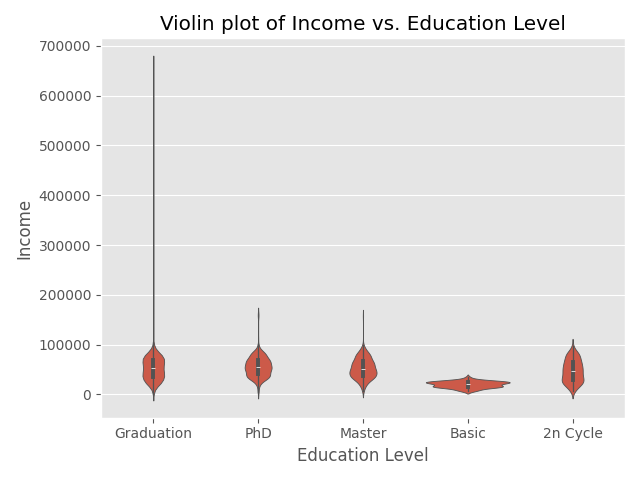
\includegraphics[width=0.7\textwidth]{./images/violin_income_vs_edu_level.png}
    \caption{Violion plot of \textit{Income} for different \textit{Education Levels}}
    \label{fig:Figure_1}
\end{figure}

\begin{figure}[H]
    \centering
    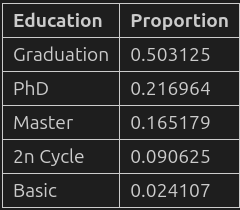
\includegraphics[width=0.5\textwidth]{./images/propotion_table_for_different_edu_levels.png}
    \caption{Propotions of different groups of \textit{Education Level} }
    \label{fig:Figure_2}
\end{figure}


\noindent \textbf{Connection of Accpeting Campaigns and Spending Behavior}: KDE plot in Figure~\ref{fig:Figure_3} shows two key points about the distribution of \textit{TotalSpendings} in different groups of customers:
\begin{itemize}
    \item First, the data in both of these two groups- namely, the ones who accepted customer campaigns and the ones who haven't.- is not normally distributed.
    \item Second, that the mean of \textit{TotalSpendings} seems to be significantly higher in the accept group than reject group.
    \item Also if we examine the propotion of the data(463 accepted vs. 1777 rejected)in the these two groups, we figure out that the data is imbalanced.
\end{itemize}

\begin{figure}[H]
    \centering
    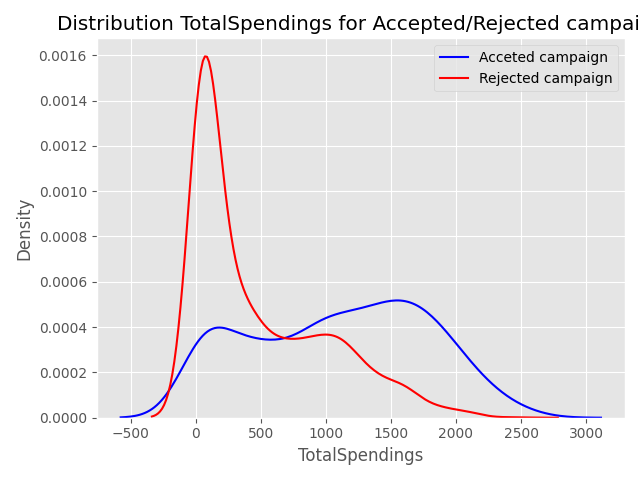
\includegraphics[width=0.7\textwidth]{./images/distro_totalspending_for_accept_reject_campaign.png}
    \caption{KDE plot of \textit{TotalSpendings} for the group of customers who accepted \textit{customer campaigns} and the ones who haven't.}
    \label{fig:Figure_3}
\end{figure}


\noindent \textbf{Impact of Having Children in Spending Behavior}: If we have a look at Figure~\ref{fig:Figure_4} which shows the KDE plot of \textit{TotalSpendings} for two different groups of customers- namely, 
those who have children, and the ones who have not-, we get two different insights similar to previous analyses:
\begin{itemize}
    \item The data in both of the groups, seems not to be normally distributed.
    \item And also, the groups without children seem to have a significantly higher median in terms of \textit{TotalSpendings}.
\end{itemize}
 
\begin{figure}[H]
    \centering
    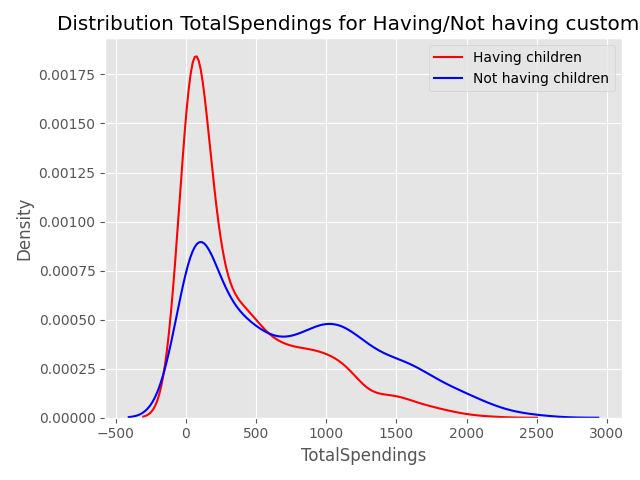
\includegraphics[width=0.7\textwidth]{./images/distro_totalspending_for_having_not_having_customers.png}
    \caption{KDE plot of \textit{TotalSpendings} for customers with and without children.}
    \label{fig:Figure_4}
\end{figure}


\noindent \textbf{Relationship of Product Category and Spendings}: If we have a look Figure~\ref{fig:Figure_5}, which shows the Parallel Coordinates plot of \textit{Spendings} for different product categories, 
we can say that there is a significant difference between \textit{Spendings} of different categories.

\begin{figure}[H]
    \centering
    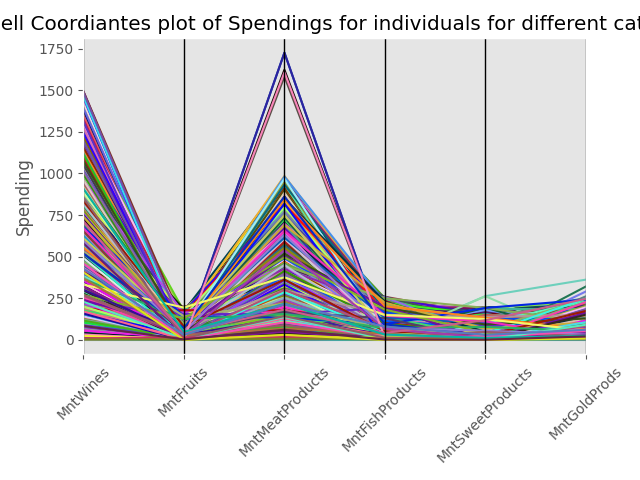
\includegraphics[width=0.7\textwidth]{./images/parallel_coor_spending_indivi_category.png}
    \caption{Parallel Coordinates plot of \textit{Spendings} for different \textit{product categories}.}
    \label{fig:Figure_5}
\end{figure}


\noindent \textbf{Impact of Education Level on Acceptance of Campaigns}: By having a look at Contingency Table in Figure~\ref{fig:Figure_6}, we find out that there isn't a significant in terms of \textit{Acceptance}, 
for different groups of \textit{Education Level}. We also see that all entries in the Expected Contingency Table(Figure~\ref{fig:Figure_7}) of these two variables have a expected frequency higher than 5.

\begin{figure}[H]
    \centering
    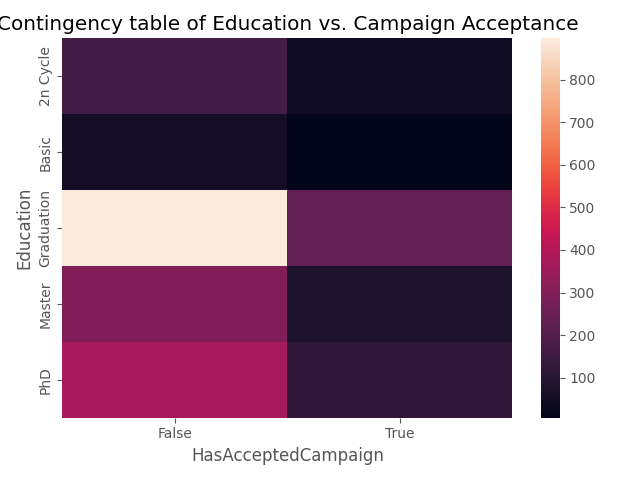
\includegraphics[width=0.8\textwidth]{./images/contingency_edu_vs_campaign_acceptance.png}
    \caption{Contingency Table of \textit{Education Level} and \textit{Campaign Acceptance}}
    \label{fig:Figure_6}
\end{figure}

\begin{figure}[H]
    \centering
    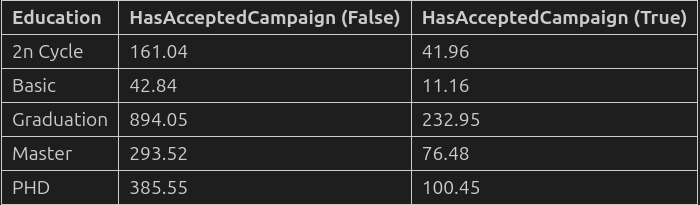
\includegraphics[width=0.8\textwidth]{./images/expected_contingency_table_of_edu_level_and_accept_reject_campaign.png}
    \caption{Expected Contingency Table of \textit{Education Level} and \textit{accept/reject campaign groups}}
    \label{fig:Figure_7}
\end{figure}


\subsubsection*{Furthur Analysis} 
\noindent \textbf{What and Why to analyze further}: Our analysis of \textbf{Connection of Accpeting Campaigns and Spending Behavior} shown us that there is an strong relationship between these two, 
And this could actually be an important result of our analysis which shows the effectiveness of our business in terms of growing the \textit{Spending Bahvior} for the customers that have accepted to be in the \textit{customer campaigns}. 
This motivates to do more investigations and ask questions about the measure of sucess of the business in terms of adverstisement. Therefore, we would like to add analysis of \textbf{Impact of Campaign Acceptance on Number of Deal Purchases} to our work. \\

\noindent \textbf{Impact of Campaign Acceptance on Number of Deal Purchases}: First, we have to note from our prior analysis \textbf{Connection of Accpeting Campaigns and Spending Behavior}, that the data is imbalanced here and we have to take this into consideration because it affects our interpretation here, in this analysis. 
Therefore, we decide to solve this problem by under sampling in the reject group. We get a better, more practial view of how the data is distributed in these two groups.
By looking at the Histograms in Figure~\ref{fig:Figure_8}, we find out that the business has not been effective in terms of growing the \textit{Number of Deals Purchases} in the \textit{accept group}, since there is no cutting eye difference between the distributions.

\begin{figure}[H]
    \centering
    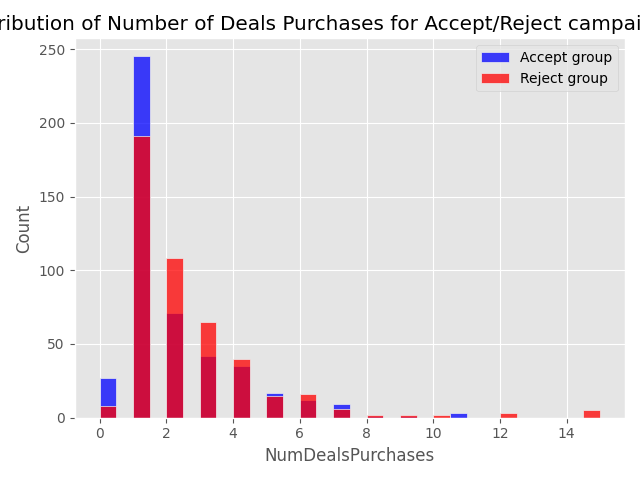
\includegraphics[width=0.7\textwidth]{./images/distro_num_of_deal_purchases_accept_reject_campaign.png}
    \caption{Distribution of \textit{Number of Deals Purchases} for \textit{accept/reject group}}
    \label{fig:Figure_8}
\end{figure}

% \subsection*{Insights and Discussion}
% \noindent \textbf{}: dsada \\ 
% \noindent \textbf{}: dsada \\ 
% \noindent \textbf{}: dsada \\ 
% \noindent \textbf{}: dsada \\ 
% \noindent \textbf{}: dsada \\ 
% \noindent \textbf{}: dsada \\ 

% \item Do customers from different education levels have different income levels?
%     \item Does the marketing campaign influence spending behavior across customer
%     groups?
%     \item Do customers with children spend differently than those without children?
%     \item Is there a significant difference in spending on different product categories?
%     \item Is there a relationship between customer education level and acceptance
%     of promotional campaigns?

\subsection*{Discussion on the Methodologies to be used:}
\textbf{Now, we should specify what statistical test to use for each of the hypothesis, the correct order to test the hypothesses and discuss why:}
\begin{enumerate}
    \item Does the marketing campaign influence spending behavior across customer groups? \( \rightarrow \) \textbf{Mann-Whitney U test}. Based on our prior analysis in EDA section, 
    we see that these two groups are not normally distributed in terms of \textit{TotalSpendings}, and also the data is imbalanced. Thus the assumptions of \textbf{two sample t-test} don't hold. Therefore we should run \textbf{Mann-Whitney U test}.

    \item Have our buisness been effective in terms of motivating customers in the campaigns to go towards deals purchasing? \( \rightarrow \) \textbf{Mann-Whitney U test}. Based on what we saw in Figure~\ref{fig:Figure_8}, 
    we can say that the data in these two group of customers is not normally distributed. Also the data is moderately imbalanced, Thus the assumptions of \textbf{two sample t-test} don't hold and we must perform \textbf{Mann-Whitney U test}.

    \item Do customers from different education levels have different income levels? \( \rightarrow \) \textbf{Kruskal-Wallis H test}. From what we saw in earlier analysis in EDA section, 
    we figured out that the groups are not normally disributed in terms of \textit{Income} and are imbalanced as well, Thus the assumptions of \textbf{ANOVA one-way test} don't hold. Therefore we should perform \textbf{Kruskal-Wallis H test}.  
    
    \item Is there a relationship between customer education level and acceptance of promotional campaigns? \( \rightarrow \) \textbf{\( \chi^2\:-independence\:test \)}. Based on what we saw in Figure~\ref{fig:Figure_7} in our prior analysis in EDA, 
    see that the least frequency assumption of \textbf{\( \chi^2\:-independence\:test \)} holds. Therefore we can perform this test.

    \item Do customers with children spend differently than those without children? \( \rightarrow \) \textbf{Mann-Whitney U test}. In our last analysis of this matter in EDA section, 
    we saw that the data in these two groups of customers is not normally distributed, Thus the normality assumption of \textbf{two sample t-test} doesn't hold. Therefore we must perform \textbf{Mann-Whitney U test}.

    \item Is there a significant difference in spending on different product categories? \( \rightarrow \) \textbf{Friedman test}. Since the distribution of \textit{Spendings} for different \textit{Product Categories} might not follow a normal distribution.
    Thus, we must perform \textbf{Friedman test} instead of \textbf{ANOVA repeated-measures test}.
\end{enumerate} 


% ----------------------------------------------------------------------------------------------------------------------------------------------------------------------------------------------------------------------

\section*{Hypothesis Testing}

\subsection*{1. Does the marketing campaign influence spending behavior across customer groups?}
\noindent \textbf{Test Used}: \textbf{Mann-Whitney U test} (\textit{alternative hypothesis: customers who have accepted campaigns, have a higher spending than customers who have not accepted campaigns.})\\ 

\noindent \textbf{Results}: Mann-Whitney U statistic: 628493.500, P-value: 0.000. \\ 

\noindent \textbf{Interpretation and Discussion}: We obtained a near-zero p-value which actually matches with our analysis in EDA section. This tells us that there is a significant difference between these two groups of customers in terms of \textit{TotalSpendings}. \\ 

\subsection*{2. Have our buisness been effective in terms of motivating customers in the campaigns to go towards deals purchasing?}
\noindent \textbf{Test Used}: \textbf{Mann-Whitney U test}. (\textit{alternative hypotheis: customers who have accepted campaigns have a lower \textit{Number of Deals Purchases} than customers who haven't accepted campaigns})\\ 

\noindent \textbf{Results}: Mann-Whitney U statistic: 340665.000, P-value: 0.000. \\ 

\noindent \textbf{Interpretation and Discussion}: We have again obtained an extremely low p-value. That matches with our prior analysis in EDA section as well. Therefore we accept the \textit{alternative hypotheis}. \\ 

\subsection*{3. Do customers from different education levels have different income levels?}
\noindent \textbf{Test Used}: \textbf{Kruskal-Wallis H test} (\textit{alternative hypothesis: customers from different education levels have different income levels.})\\ 

\noindent \textbf{Results}: Kruskal-Wallis H statistic: 142.467, P-value: 0.000. \\ 

\noindent \textbf{Interpretation and Discussion}: The extremely low p-value indicates a significant difference in income levels across different education levels, which is consistent with our earlier analysis in the EDA section. We conclude that \textbf{Education Level} does have a significant effect on \textbf{Income Level}.

\subsection*{4. Is there a relationship between customer education level and acceptance of promotional campaigns?}
\noindent \textbf{Test Used}: \textbf{Chi-Squared independence test} (\textit{alternative hypothesis: there is a relationship between education level and acceptance of campaigns.})\\ 

\noindent \textbf{Results}: Chi-Square Statistic: 5.865, P-value: 0.209. \\ 

\noindent \textbf{Interpretation and Discussion}: The p-value of 0.209 is high, indicating that there is no significant relationship between education level and campaign acceptance. This matches our previous observations in the EDA section, where we didn’t find any strong correlation between these two variables.

\subsection*{5. Do customers with children spend differently than those without children?}
\noindent \textbf{Test Used}: \textbf{Mann-Whitney U test} (\textit{alternative hypothesis: customers with children spend less than customers without children.})\\ 

\noindent \textbf{Results}: Mann-Whitney U statistic: 937520.000, P-value: 0.000. \\ 

\noindent \textbf{Interpretation and Discussion}: We obtained a very low p-value, which indicates that there is a significant difference in spending between customers with and without children. Specifically, \textbf{customers without children} tend to have \textbf{higher total spending} than those with children, as confirmed by our earlier EDA analysis.

\subsection*{6. Is there a significant difference in spending on different product categories?}
\noindent \textbf{Test Used}: \textbf{Friedman Test} (\textit{alternative hypothesis: there is a significant difference in spending across different product categories.})\\ 

\noindent \textbf{Results}: Friedman Test Statistic: 5967.749, P-value: 0.000. \\ 

\noindent \textbf{Interpretation and Discussion}: The p-value is extremely low, indicating a significant difference in spending across different product categories. This result aligns with our EDA analysis, where we saw notable variations in spending patterns depending on the product category, suggesting that customers allocate their spending differently across various products.

% ----------------------------------------------------------------------------------------------------------------------------------------------------------------------------------------------------------------------

\section*{Conclusion}
\noindent \textbf{Effectiveness of businesss in growth of \textit{Spending Behaviors}}: Based on our analysis on \textbf{Connection of Accpeting Campaigns and Spending Behavior} in EDA, and furthur 
investigation in Hypothesis Testing section, We can conclude that our business has been effective in the growing \textit{Spending Behaviors} for the \textit{customer campaigns}. \\ 

\noindent \textbf{Weakness in having affect on the \textit{Number of Deals Purchases} factor}: Our findings in \textbf{Furthur Analysis} section, and the statistcal testing that we have performed for examining our hypothesis, 
we has shown us that our buisness has weakness in terms of motivating \textit{customer campaigns} to increase their \textit{Number of Deals Purchases}. Taking against in order to increase the sales of the business by adverstisement for this group of customers could be very effective, 
since we have just concluded that this group of customers have a significantly higher \textit{TotalSpendings}. \\ 

\noindent \textbf{Education doesn't effect Campaign Acceptance}: Analysis on \textbf{Impact of Education Level on Acceptance of Campaigns}, has shown that we shouldn't pay attention to the \textit{Education Level} of the customers while we want to advertise joining the \textit{customer campaigns}. \\ 

\noindent \textbf{It matters what product we do advertise}: From our studies on \textbf{Relationship of Product Category and Spendings} in EDA section, followed by statisical testing in Hypothesis Testing section, 
We infer that it some \textit{product categories} have a significantly higher \textit{Spending}. Thus this need to be noted while advertising products. \\ 

% ----------------------------------------------------------------------------------------------------------------------------------------------------------------------------------------------------------------------

\section*{Decission Making}
\noindent \textbf{Suggestion for growing \textit{Spending Behavior} of the customers}: Based on the \textbf{Conclusion} section, understanding and the knowledge that we have obtained from this study, we have several sugesstions to make:
\begin{enumerate}
    \item We should shift our focus in advertisement of \textit{product categories}, to a more narrow, certain range of products which have a significant higher \textit{Spendings}.
    \item We must care more about the growth of \textit{Number of Deals Purchases} in the \textit{customer campaigns} of the business. Since this group has a significantly higher \textit{TotalSpendings} compared to other customers.
    \item It's good to give a raise to the employees, who have been involved in our prior programs which contributed to a growth in \textit{Spending Behaviors} inside the \textit{customer campaigns}, since their work has been effective.
\end{enumerate} 

\end{document}
